\documentclass[a4paper,14pt]{article}
\usepackage{float}
\usepackage{extsizes}
\usepackage{amsmath}
\usepackage{amssymb}
\everymath{\displaystyle}
\usepackage{geometry}
\usepackage{fancyhdr}
\usepackage{multicol}
\usepackage{graphicx}
\usepackage[brazil]{babel}
\usepackage[shortlabels]{enumitem}
\usepackage{cancel}
\columnsep=2cm
\hoffset=0cm
\textwidth=8cm
\setlength{\columnseprule}{.1pt}
\setlength{\columnsep}{2cm}
\renewcommand{\headrulewidth}{0pt}
\geometry{top=1in, bottom=1in, left=0.7in, right=0.5in}

\pagestyle{fancy}
\fancyhf{}
\fancyfoot[C]{\thepage}

\begin{document}
	
	\noindent\textbf{8FMA31~Matemática} 
	
	\begin{center}Regra de três composta - Três variáveis (Versão estudante)
	\end{center}
	
	\noindent\textbf{Nome:} \underline{\hspace{10cm}}
	\noindent\textbf{Data:} \underline{\hspace{4cm}}
	
	%\section*{Questões de Matemática}
	
	\begin{center}
		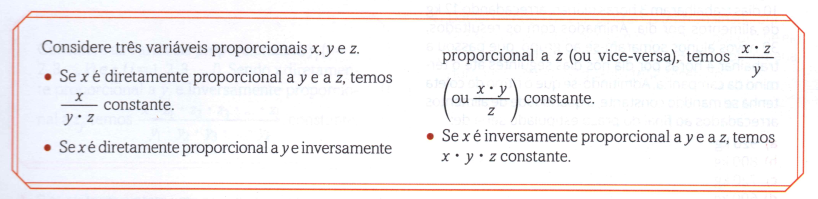
\includegraphics[width=1\linewidth]{8FMA31_imagens/imagem1}
	\end{center}
	
	
	\begin{multicols}{2}
		\begin{enumerate}
			\item (Enem) Uma confecção possuía 36 funcionários, alcançando uma produtividade de 5400 camisetas por dia, com uma jornada de trabalho de área dos funcionários de 6 horas. Entretanto, com o lançamento da nova coleção e de uma nova campanha de marketing, o número de encomendas cresceu de forma acentuada, aumentando a demanda diária para 21600 camisetas. Buscando atender essa nova demanda, a empresa aumentou o quadro de funcionários para 96. Ainda assim a carga horária de trabalho necessita ser ajustada. Qual deve ser a nova jornada de trabalho diária dos funcionários para que a empresa consiga atender a demanda?
			\begin{enumerate}[a)]
				\item 1 hora e 30 minutos.
				\item 2 horas e 15 minutos.
				\item 9 horas.
				\item 16 horas.
				\item 24 horas. \\\\\\\\\\\\\\\\\\\\\\\\\\\\\\\\\\\\\\\\\\\\\\\\\\
			\end{enumerate}
		    \item Cinco coelhos comem 20 cenouras em 12 minutos. Em quantos minutos 15 coelhos comeriam 50 cenouras? \\\\\\\\\\\\\\\\\\\\\\\\\\\\
		    
		    \item (Enem) Uma indústria tem um setor totalmente automatizado. São quatro máquinas iguais que trabalham simultânea e ininterruptamente durante uma jornada de 6 horas. Após esse período, as máquinas são desligadas por 30 minutos para manutenção. Se alguma máquina precisar de mais manutenção, ficará parada até a próxima manutenção. Certo dia, era necessário que as quatro máquinas produzissem um total de 9000 itens. O trabalho começou a ser feito às 8 horas. Durante uma jornada de 6 horas produziram 6000 itens, mas na manutenção observou-se que uma máquina precisava ficar parada. Quando o serviço foi finalizado as três máquinas que continuaram operando passaram por uma nova manutenção, chamada manutenção de esgotamento. Em que horário começou a manutenção de esgotamento?
		    \begin{enumerate}[a)]
		    	\item 16h45min
		    	\item 18h30min
		    	\item 19h50min
		    	\item 21h15min
		    	\item 22h30min \\\\\\\\\\\\\\\\\\\\\\\\\\\\\\\\\\\\\\\\\\\\\\\\\\\\\\\\\\\\
		    \end{enumerate}
	    	\item (Enem) Uma escola lançou uma campanha para seus alunos arrecadarem, durante 30 dias, alimentos não perecíveis para doar a uma comunidade carente da região. Vinte alunos aceitaram a tarefa e nos primeiros 10 dias trabalharam 3 horas diárias, arrecadando 12 kg de alimentos por dia. Animados com os resultados, 30 novos alunos somaram-se ao grupo, que passou a trabalhar 4 horas por dia nos dias seguintes até o término da campanha.
	    	Admitindo-se que o ritmo de coleta tenha se mantido constante, a quantidade de alimentos arrecadados ao final do prazo estipulado seria de:
	    	 \begin{enumerate}[a)]
	    		\item 920 kg
	    		\item 800 kg
	    		\item 720 kg
	    		\item 600 kg
	    		\item 570 kg \\\\\\\\\\\\\\\\\\\\\\\\\\\\\\
	    	\end{enumerate}
    	    \item Com um galão de tinta, pode se pintar uma escultura de 4 metros de altura. Quantos galões de tinta seriam necessários para pintar 350 esculturas semelhantes, com a metade da altura? \\\\\\\\\\\\\\\\\\\\\\\\\\\\\\\\\\\\\\\\\\\\\\\\\\\\\\\\\\\\\\\\\\\\
    	    \item Numa confecção de roupas, seis costureiras fazem 18 calças em 10 horas. Considerando que todas as costureiras possuem o mesmo rendimento, responda:
    	    \begin{enumerate}[a)]
    	    	\item Nesse tempo, quantas calças são feitas por quatro costureiras? \\\\\\\\\\\\\\\\\\\\\\\\\\\\\\
    	    	\item Para fazer as mesmas 18 calças, de quanto tempo 8 costureiras necessitam? Dê sua resposta em horas e minutos. \\\\\\\\\\\\\\\\\\\\\\\\
    	    	\item Em quanto tempo uma costureira faz uma calça? Dê sua resposta em horas e minutos. \\\\\\\\\\\\\\\\\\\\\\\\\\\\\\
    	    \end{enumerate}
            \item Três torneiras de mesma vazão enchem uma caixa d’água de 1200 litros em 80 minutos. Quantas torneiras idênticas às anteriores serão necessárias para encher quatro caixas d'água de 600 litros em uma hora? \\\\\\\\\\\\\\\\\\\\\\\\\\\\\\
            
            \item Considere em cada item, que todos os professores de uma escola tem o mesmo ritmo de trabalho.
            \begin{enumerate}[a)]
            	\item Um professor leva 2:30 para corrigir 120 provas. Quantas provas ele corrige em 20 minutos? \\\\\\\\\\\\\\\\\\\\\\\\\\
            	\item Quatro professores levam 5 horas para corrigir algumas provas. Quanto tempo seis professores levariam para corrigir as mesmas provas? \\\\\\\\\\\\\\\\\\\\\\\\\\\\\\\\
            	\item Três professores corrigem 700 provas em 6 horas quantas provas sete professores corrigem em 9 horas? \\\\\\\\\\\\\\\\\\\\\\\\\\
            \end{enumerate}
            \item Numa gráfica, três impressoras idênticas imprimem 30000 páginas a cada 6 horas. Quantas impressoras iguais a essas são necessárias para imprimir 45.000 páginas em 3 horas?
		\end{enumerate}
	$~$ \\ $~$ \\ $~$ \\ $~$ \\ $~$ \\ $~$ \\ $~$ \\ $~$ \\ $~$ \\ $~$ \\ $~$ \\ $~$ \\ $~$ \\ $~$ \\ $~$ \\ $~$ \\ $~$ \\
    \end{multicols}
\end{document}